\documentclass[sigconf,nonacm]{acmart}

\usepackage{subcaption}

\setcopyright{none}

\begin{document}

\title{Programming III --- project report}

\author{Ivan Mikhailov}
\affiliation{
  \institution{University of Primorska (FAMNIT)}
  \city{Koper}
  \country{Slovenia}
}
\email{89231117@student.upr.si}

\maketitle

\section{Introduction}
The topic I chose is called “Factorio Throughput Calculator.” It is a simplified simulation of production lines with a predefined layout. The simulation ends automatically when resources have not moved for 5 ticks.

\section{Implementation}
I developed three versions of this application: sequential, multithreaded, and distributed.
They all share the same structure and were developed sequentially in a single Git repository.

\section{Tiles and sprites}
I drew the sprites for the tiles myself in a computer editor; the images are schematic. The sprites for each tile are shown in Figure~\ref{fig:sprites}, and their behaviour is described below.

\begin{figure}[h]
  \centering
  \begin{subfigure}{0.23\linewidth}
    
\includegraphics[width=\linewidth]{sprites/source-iron}
    \caption{Iron source}
  \end{subfigure}
  \begin{subfigure}{0.23\linewidth}
    
\includegraphics[width=\linewidth]{sprites/source-copper}
    \caption{Copper source}
  \end{subfigure}
  \begin{subfigure}{0.23\linewidth}
    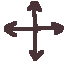
\includegraphics[width=\linewidth]{sprites/conveyor}
    \caption{Conveyor belt}
  \end{subfigure}
  \begin{subfigure}{0.23\linewidth}
    
\includegraphics[width=\linewidth]{sprites/splitter}
    \caption{Splitter}
  \end{subfigure}

  \vspace{0.5em}
  \begin{subfigure}{0.23\linewidth}
    
\includegraphics[width=\linewidth]{sprites/assembler1}
    \caption{Assembling station 1}
  \end{subfigure}
  \begin{subfigure}{0.23\linewidth}
    
\includegraphics[width=\linewidth]{sprites/assembler2}
    \caption{Assembling station 2}
  \end{subfigure}
  \begin{subfigure}{0.23\linewidth}
    
\includegraphics[width=\linewidth]{sprites/chest}
    \caption{Chest}
  \end{subfigure}
  \begin{subfigure}{0.23\linewidth}
    
\includegraphics[width=\linewidth]{sprites/empty}
    \caption{Empty}
  \end{subfigure}
  \caption{Sprites used for each tile type.}
  \Description{A grid of eight hand-drawn schematic icons, one per tile type: an iron source and a copper source, each shown as a two-letter monogram; a conveyor belt shown as a four-way arrow; a splitter shown as an arrow branching into two; assembling station 1 and assembling station 2, each shown as a number; a chest shown as a small box; and an empty tile shown as a plain square.}
  \label{fig:sprites}
\end{figure}

\begin{description}
  \item[Source] Generates one resource of a fixed type (iron or copper) per tick and holds up to a configurable number of items internally. Each tick, it attempts to push one item to every neighbouring tile that can accept it. The two variants shown are distinguished by the letters \textit{SI} (iron) and \textit{SC} (copper).
  \item[Conveyor belt] A straight belt with a fixed facing direction that can hold at most one item. Each tick, it tries to push its item onto the tile it faces, if that tile can accept it.
  \item[Splitter] A T-shaped tile with one input side and two output sides (left and right), holding at most one item. Each tick it pushes an item, it alternates between the left and right outputs, so an incoming stream is split evenly between the two sides.
  \item[Assembling station 1] Holds up to two items and only accepts copper. Once it holds two copper, it processes for two ticks, then consumes them and produces one copper wire, which it attempts to push to the tile on its right.
  \item[Assembling station 2] Only accepts iron and copper wire. Once it holds one iron and one copper wire, it processes for three ticks, then consumes them and produces one inductor, which it attempts to push to the tile on its right.
  \item[Chest] Accepts and stores an unlimited number of items; it is used to collect the final output of a production line.
  \item[Empty] Not part of the assignment's tile types, but present in my implementation as a placeholder for unused grid cells: it holds no items and cannot be crossed.
\end{description}

\section{GUI and screenshots}
The interface is built with Java Swing.

\begin{figure}[h]
  \centering
  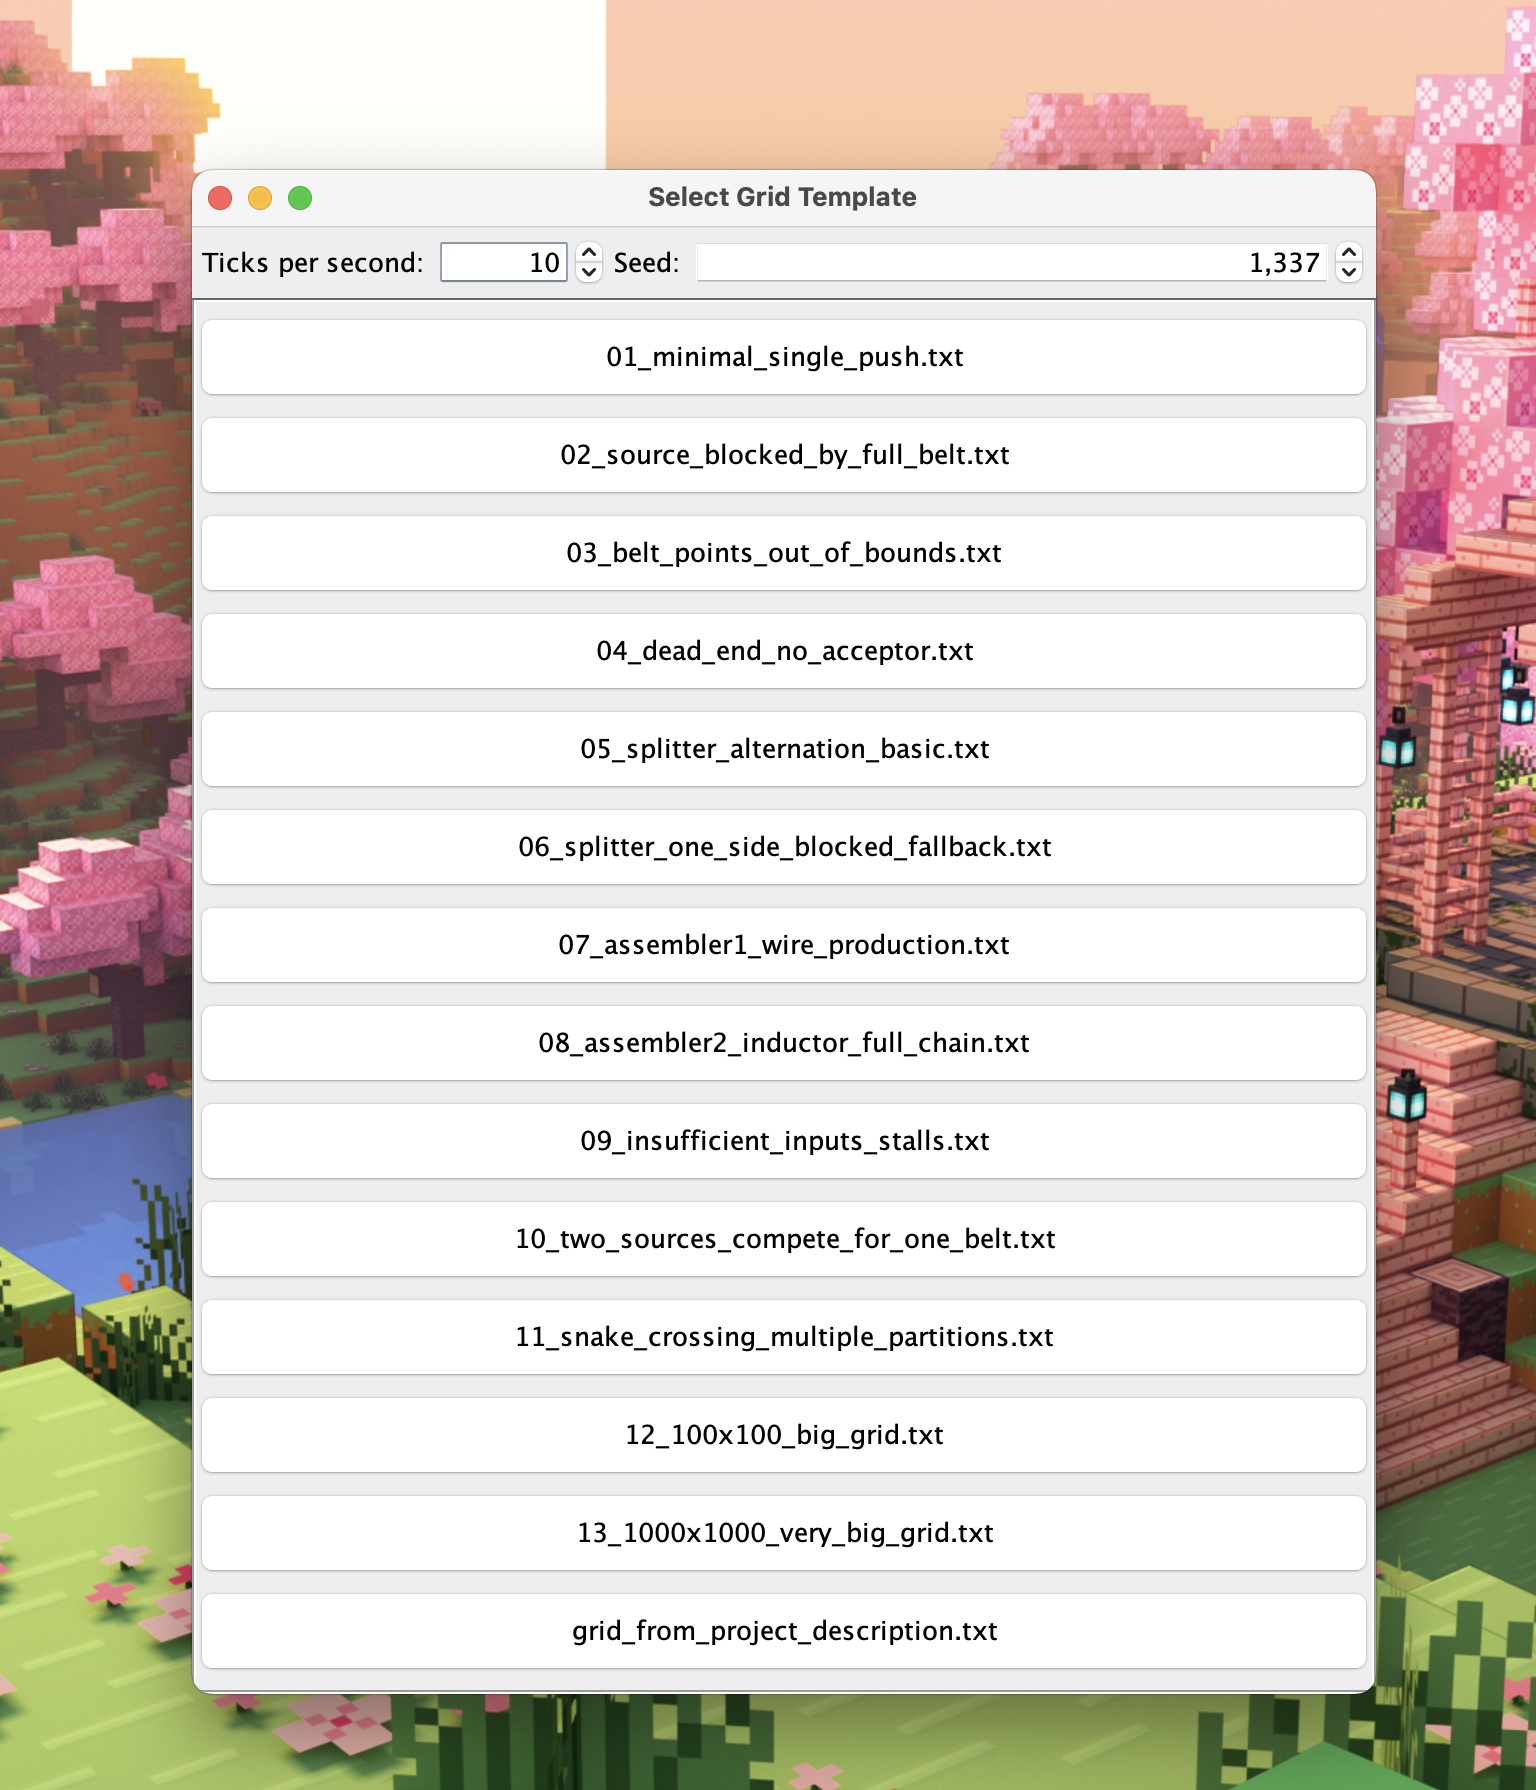
\includegraphics[width=\linewidth]{screenshots/menu}
  \caption{Grid template selection window.}
  \Description{A window listing selectable grid template files, with input fields for ticks per second and seed.}
\end{figure}

\begin{figure}[h]
  \centering
  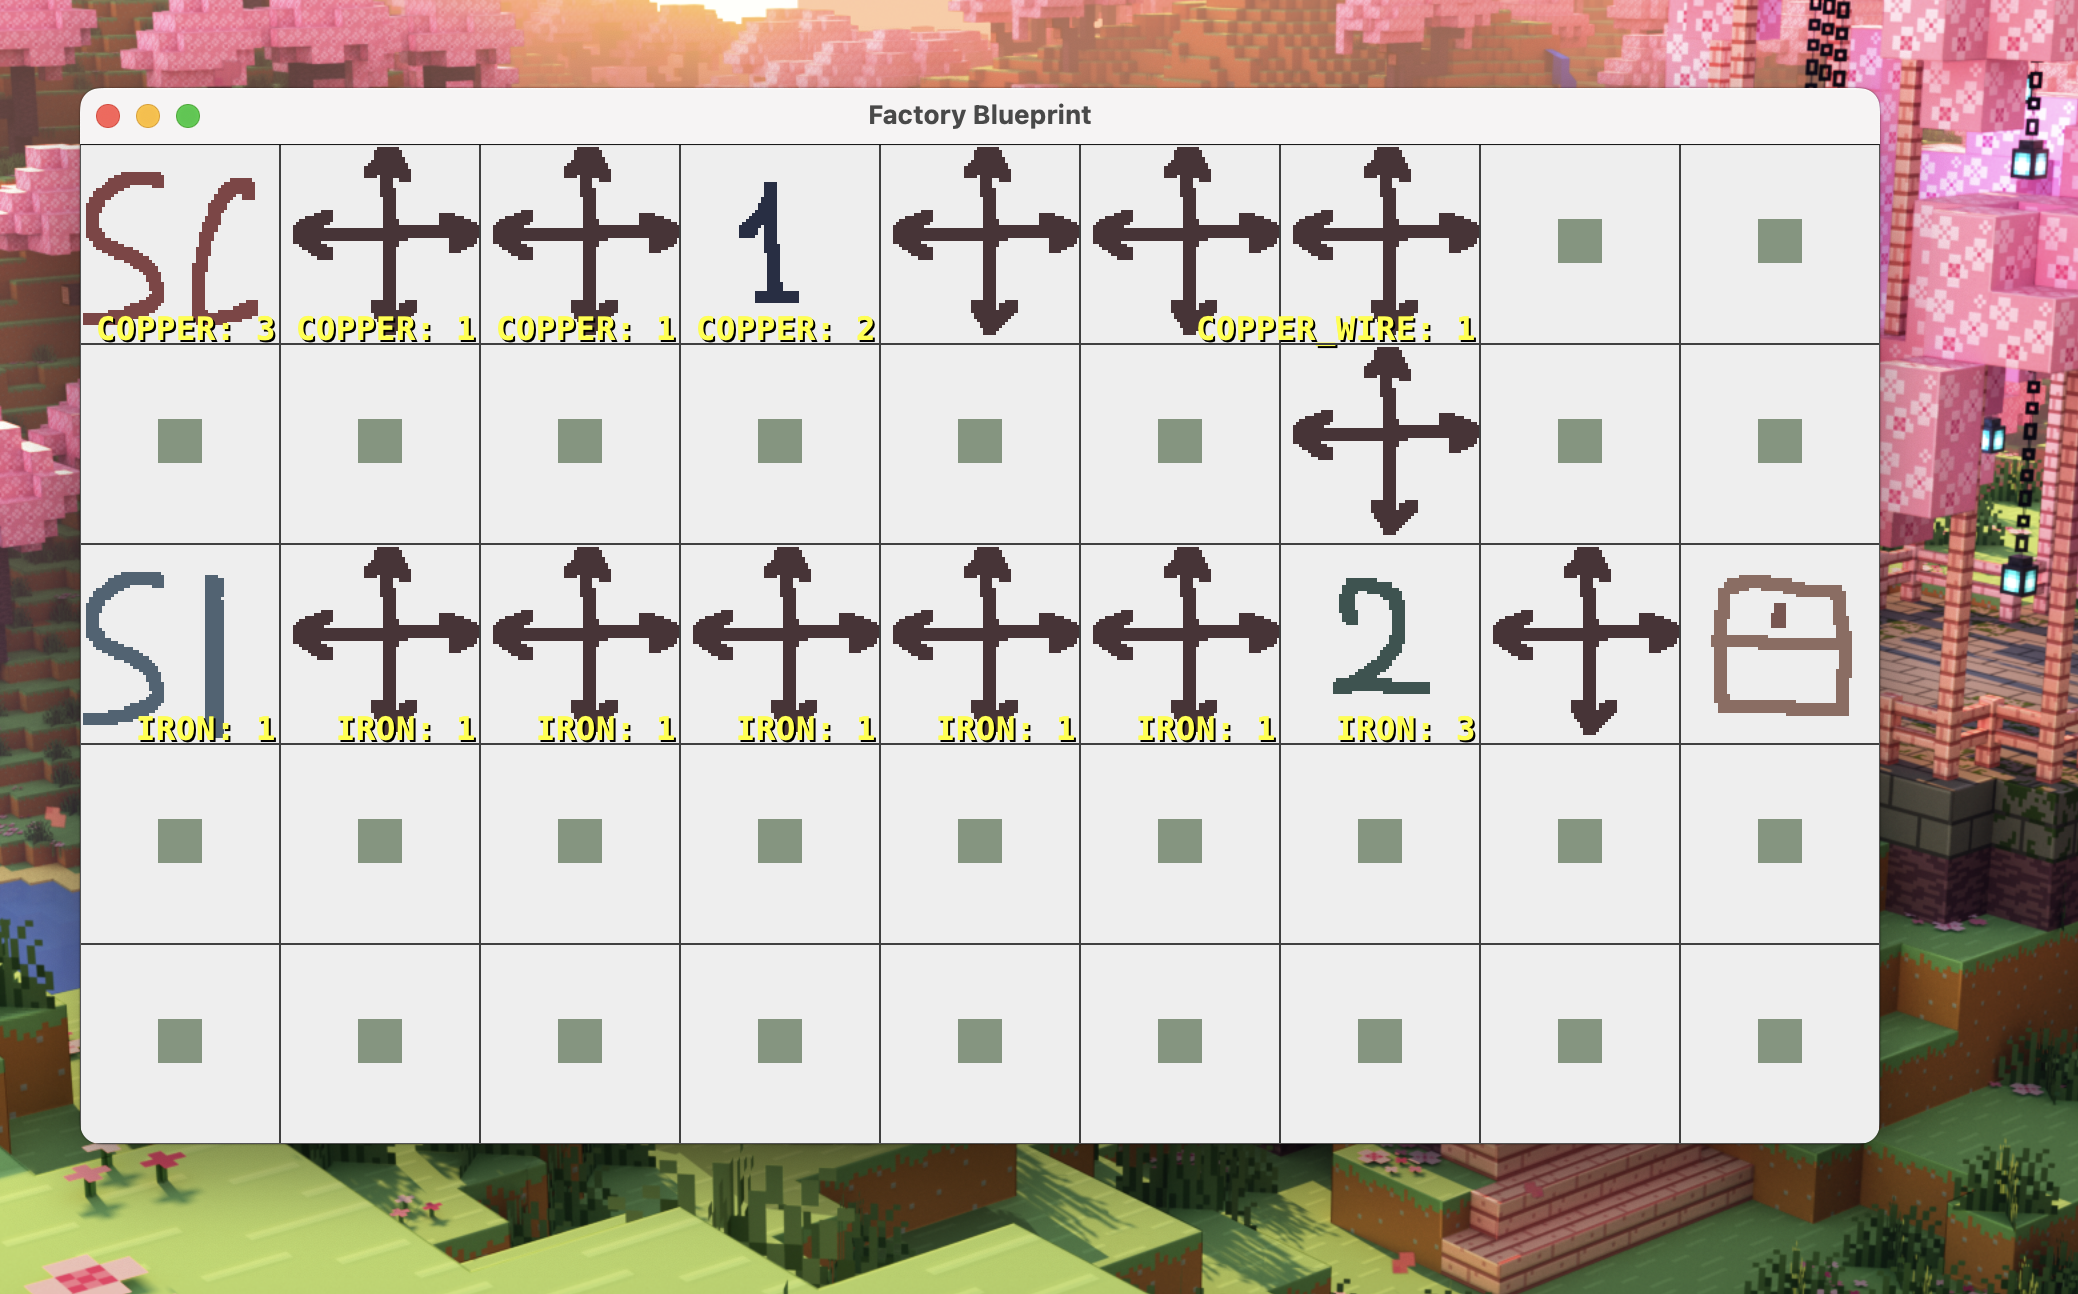
\includegraphics[width=\linewidth]{screenshots/game}
  \caption{Running simulation.}
  \Description{A grid of tiles with sprites for sources, conveyor belts, splitters, assembling stations, and a chest, each tile labelled with its current resource counts.}
\end{figure}

\begin{figure}[h]
  \centering
  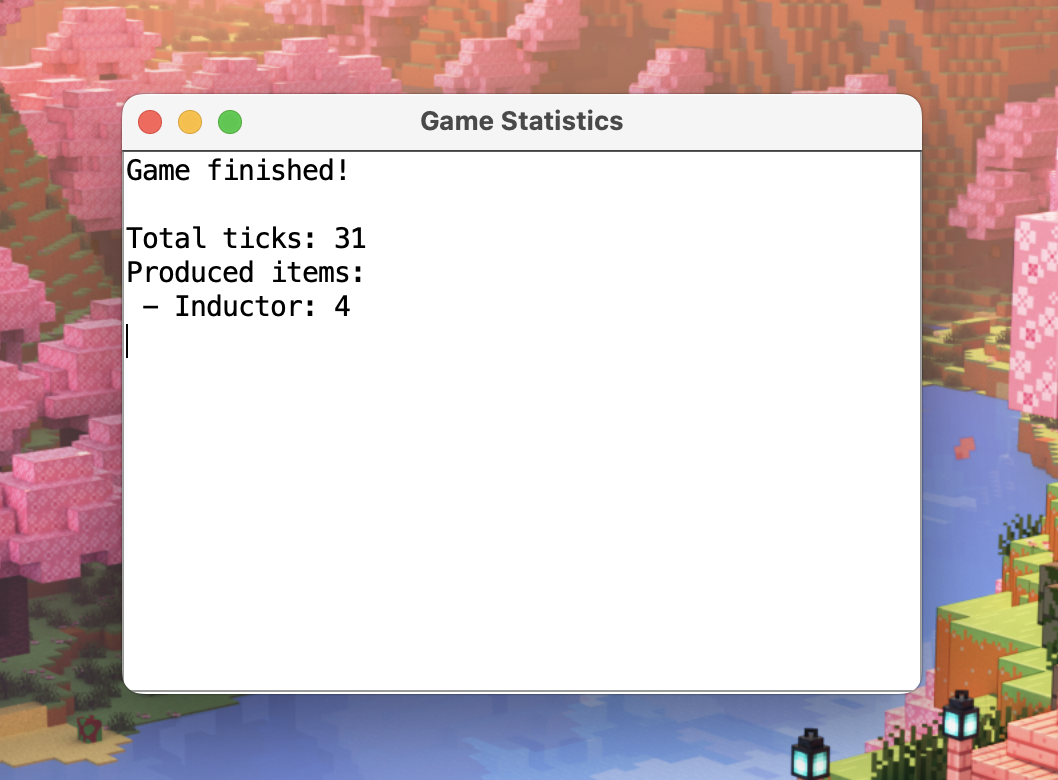
\includegraphics[width=0.7\linewidth]{screenshots/result}
  \caption{Statistics window shown after the simulation ends.}
  \Description{A window reporting the total number of ticks and the produced items after the simulation finished.}
\end{figure}

\section{Sequential solution}
is located in the \texttt{sequential} branch.
The main executable class is \texttt{src/main/java/io/github/redheadflag/engine/Main.java}

\section{Multithreaded solution}
is located in the \texttt{multithreaded} branch. The main executable class is \texttt{src/main/java/io/github/redheadflag/engine/Main.java}

\section{Distributed solution}

\subsection{Installation}
Running the distributed solution requires MPJ Express, an MPI implementation for Java, and Maven to build the project, since the compiled classes (\texttt{target/classes}) are not committed to the repository.

\begin{enumerate}
  \item \begin{sloppypar}Download MPJ Express from \url{http://mpjexpress.org/download.php} and extract it into a folder named \texttt{mpj} in the project root.\end{sloppypar}
  \item Compile the project with Maven:
\begin{verbatim}
mvn compile
\end{verbatim}
  \item MPJ is not published on Maven Central, so its jar must be installed into the local Maven repository by hand, to satisfy the \texttt{mpj:mpj:0.44} dependency declared in \texttt{pom.xml}:
\begin{verbatim}
mvn install:install-file \
  -Dfile=mpj/lib/mpj.jar \
  -DgroupId=mpj \
  -DartifactId=mpj \
  -Dversion=0.44 \
  -Dpackaging=jar
\end{verbatim}
  \item Run the simulation across \texttt{N} processes:
\begin{verbatim}
export MPJ_HOME="$(pwd)/mpj"
"$MPJ_HOME/bin/mpjrun.sh" -np N \
  -cp target/classes \
  io.github.redheadflag.engine.Main
\end{verbatim}
\end{enumerate}

\subsection{Implementation}
\begin{sloppypar}is located in the \texttt{distributed} branch. The main executable class is \texttt{src/main/java/io/github/redheadflag/engine/Main.java}, extended to initialize MPI, partition the grid's tiles across processes, and synchronize transfers across partition boundaries via message passing; only the process with rank 0 displays the GUI.\end{sloppypar}

\section{Comparison}
Measured on a machine with an Apple M4 processor (10 cores).

\begin{table}[h]
  \caption{Execution time by grid size and implementation (ms).}
  \label{tab:comparison}
  \resizebox{\linewidth}{!}{%
  \begin{tabular}{lccccc}
    \toprule
    Grid & Sequential & Multithreaded & Distributed (np=2) & Distributed (np=4) & Distributed (np=8) \\
    \midrule
    \#8 (5x9)   & \textbf{2}    & 6    & 6    & 11   & -- \\
    100x100     & \textbf{41}   & 203  & 97   & 172  & 161  \\
    1000x1000   & 6985 & \textbf{3471} & 3203 & 3741 & \textbf{3072} \\
    \bottomrule
  \end{tabular}%
  }
\end{table}

\section{Conclusion}
Based on the tests I conducted on grids of various sizes, the following conclusions can be drawn:
\begin{itemize}
  \item Parallel execution does indeed provide a speed advantage. However, this speed gain is only noticeable on large grids.
  \item Performance loss depends less on grid size than on how well it decomposes into independent components; even the mid-sized 100x100 grid loses performance under parallelism.
  \item Distributed and multithreaded are close only on the largest grid. On 100x100, distributed is clearly faster than multithreaded.
\end{itemize}

\end{document}
